\documentclass[preprint]{aastex} %double-column, single-spaced document:
%\documentclass[iop,floatfix]{emulateapj} 

\usepackage{hyperref}
%\usepackage{graphicx}
%\usepackage{apjfonts}
\usepackage{enumerate}
\usepackage{amsmath,amssymb}
\usepackage{geometry}
\usepackage{bm}
\usepackage[usenames,dvipsnames,svgnames,table]{xcolor}

\newcommand{\prob}{{\rm prob}}
\newcommand{\qN}{\{q_i\}_{i=1}^N}
\newcommand{\qM}{\{q_{im}\}_{i=1,m=0}^{N,M}}
\newcommand{\yN}{\{y_i\}_{i=1}^N}
\newcommand{\vt}{\vec{\theta}}
\newcommand{\vg}{\vt_{\star, {\rm grid}}}
\newcommand{\vpp}{\vt_{\star, {\rm post}}}
\newcommand{\vstar}{\vt_{\star}}
\newcommand{\vN}{\vt_{\rm N}}
\newcommand{\vc}{\vec{c}}
\newcommand{\fM}{ {\bm M}}
\newcommand{\fMi}{M_i}
\newcommand{\fD}{ {\bm D}}
\newcommand{\fDi}{D_i}
\newcommand{\dd}{\,{\rm d}}
\newcommand{\trans}{\mathsf{T}}
\newcommand{\Z}{[{\rm Fe}/{\rm H}]}
\newcommand{\A}{[\alpha/{\rm Fe}]}

\newcommand{\hcom}[1]{ \textcolor{Blue}{#1}}


%\slugcomment{}
%\shorttitle{}
%\shortauthors{}

\begin{document}

\title{Methods for the spectroscopic inference of fundamental stellar parameters, continued.}
\author{\today{}\\
\medskip
Ian~Czekala\altaffilmark{1} et al.
%Author2\altaffilmark{2},
}

\altaffiltext{1}{Harvard-Smithsonian Center for Astrophysics, 60 Garden Street MS 10, Cambridge, MA 02138}
%\altaffiltext{2}{Institution 2}
\email{iczekala@cfa.harvard.edu}

\section{Downsampling}

\hcom{section 2: why ``linearly interpolate?'' It would be good to see more specificity here; there are lots of ways to do this smooth and downsample slightly wrong.}

There are a few interpolations that are going on in this method. I will explain them in order.

\subsection{Interpolating a spectrum from a grid of synthetic spectra}
If we desire a raw, synthetic spectrum that has stellar properties $\vg = \{T_{\rm eff}, \log g, [{\rm Fe}/{\rm H}]\}$ that are not one of the grid points, then we must interpolate. At the moment, this is done as a linear interpolation because it is quick and memory efficient. I do agree with you that it would be better to use a more sophisticated interpolator. For example, \citet{hwd+13} use a spline interpolator that we plan to implement soon. This has currently been a low priority because our interpolation tests show that the expected error due to this interpolation should be small. However, for each raw pixel of the spectrum, we \emph{should} be doing a band-limited interpolation with respect to $T_{\rm eff}$, $\log g$, and $[{\rm Fe}/{\rm H}]$.

After interpolation, the new spectrum we just interpolated from the grid has the same pixel spacing and resolution as the original synthetic spectra.

\hcom{When you do the drop and interpolate over testing, can you build an empirical interpolation error model and then use it?}
Point taken! It's on the to-do list.

\subsection{Post-processing the interpolated raw spectrum into one that can be compared to our data spectrum}

We flux-calibrate our data spectrum by comparison with a spectrophotometric standard. Using the IRAF tasks \texttt{standard}, \texttt{sensfunc}, and \texttt{calibrate}, we convert the raw spectrum (in units of counts/pixel) into a flux-density ($f_\lambda$ in units of ${\rm erg}/{\rm s}/{\rm cm}^2/$\AA) by dividing by the sensitivity function determined from the spectrophotometric standard.

The raw synthetic spectra are also given in spectral flux density ($f_\lambda$), sampled at $R\approx$500,000. I prefer to think of the synthetic spectrum as a band-limited function that is sampled at many points, hopefully fine enough such that it is Nyquist sampled. Stellar spectra in particular are band-limited by several effects. The first is that intrinsic stellar phenomenon like microturbulence, macroturbulence, and rotation all act to suppress high frequency features in the spectrum.  Second, the line-spread function of the observing instrument also removes high frequency stellar features. Finally, the width of the pixel on the CCD also destroys spectral information of the highest frequencies, if any remain. The result is that a band-limited spectrum has a Nyquist frequency above which we need not sample, but below which we sample at our peril.

To transform our raw interpolated spectrum into a format that matches our data spectrum, we first resample the uniformly sampled (in angstroms) raw spectrum to a log-linear wavelength grid using spline interpolation. We take care to use a fine enough spacing such that no spectral information is lost. We test that we can interpolate from the log-linear grid \emph{back} to the original grid and recover the same flux values to within floating point accuracy. A log-linear grid has constant spacing in velocity space, and so it is the appropriate grid to use for an FFT. Once in Fourier space, we then multiply the spectrum by the PSF kernel of the instrument and a $v \sin i$ kernel for rotational broadening. For an illustration of the effects on the spectrum in Fourier space, see Figure~\ref{fig:pixel_response}.

\begin{figure}[!htb]
\begin{center}
  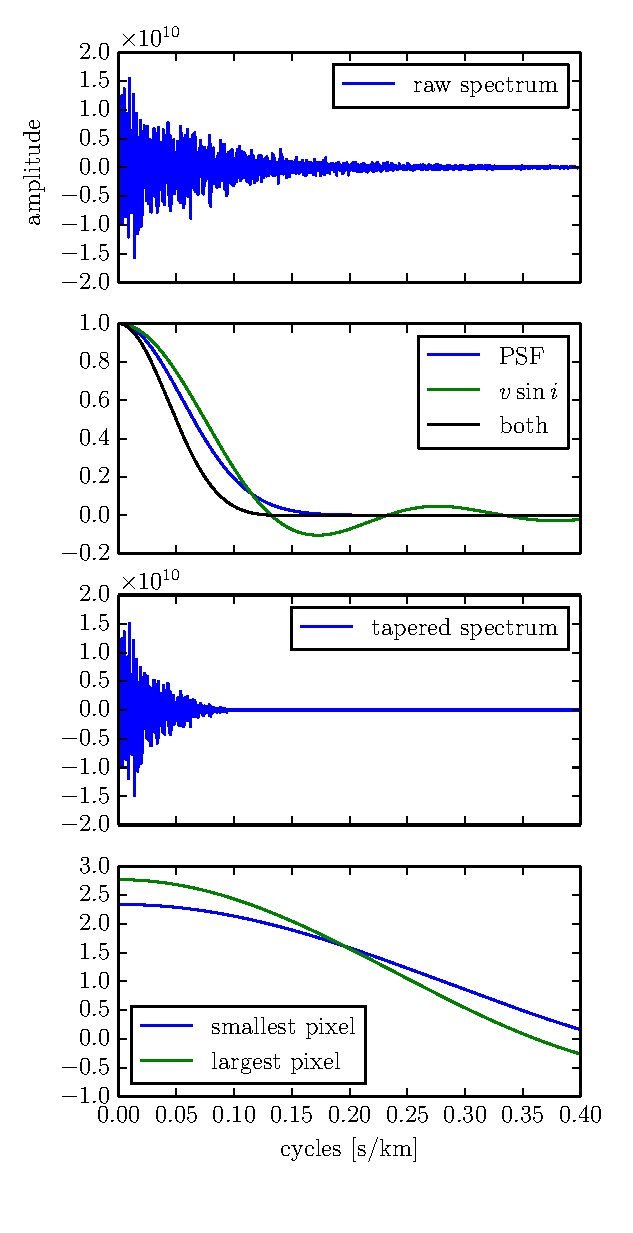
\includegraphics[width=0.48\textwidth]{pixel_response}
  \caption{What happens to the spectrum in the Fourier domain during post processing. The first panel shows the Fourier transform of the raw spectrum interpolated from the grid. The second panel shows the kernels for a PSF with ${\rm FWHM} = 6.8$ km/s and a rotation kernel for $v\sin i = 5$ km/s. The third panel is the raw spectrum multiplied by these kernels. The final panel shows the sinc functions representing the frequency response of the smallest and largest pixel on our detector.}
\label{fig:pixel_response}
\end{center}
\end{figure}

Should we be accounting for pixel effects? In the image plane, an individual pixel could be represented as a box-car or top-hat function which convolves the spectrum $f_\lambda$ and is then resampled at the pixel-center $\lambda_0$. In the Fourier domain, the effect of the pixel is represented as multiplication by a sinc function. Because the width of the pixel is small, the main lobe of the sinc function is large. Figure~\ref{fig:pixel_response} shows that all of the stellar information in Fourier space is within this main lobe, and so as an approximation it seems like we do not need to worry about pixel-convolutions. I believe the situation would be different if our pixels undersampled the PSF. 

Ignoring the pixel width effects for now, we do an IFFT back to the wavelength domain and then use splines to resample the flux-density at the exact pixel centers of our dataset. Here, we also test the spline interpolation using differently spaced wavelength grids to check that we can still recover the same spectrum to within numerical accuracy. The pixels of our particular CCD are roughly log-linear spaced, and there are at least 2.5 pixels across the FWHM of the spectrograph PSF. Summarizing the previous statements in math, we have discrete samples of some synthetic stellar spectrum $f_{\lambda, {\rm synth}}$, and we would like to morph them into samples of a different spectrum $f_{\lambda, {\rm inst}}$, which correspond to the CCD pixels of our spectrograph. In wavelength space this operation is written as
\begin{equation}
  f_{\lambda, {\rm inst}}(\lambda) = \Pi(\lambda) \otimes g_{\rm PSF}(\lambda) \otimes g_{v \sin i}(\lambda) \otimes f_{\lambda, {\rm synth}}(\lambda)
  \label{eqn:convolution}
\end{equation}
and in Fourier space as
\begin{equation}
  F_{\lambda, {\rm inst}}(s) = {\rm sinc}(s) G_{\rm PSF}(s) G_{v \sin i}(s) F_{\lambda, {\rm synth}}(s)
\end{equation}


In the future, we may consider doing away with the FFT routine entirely in favour of a sliding convolution approach in the wavelength domain (Equation~\ref{eqn:convolution}). With this approach, we can account for the variation of PSF and pixel size with wavelength. The difficulty in implementation comes with implementing a continuous convolution using discrete samples of the spectrum while preserving accuracy. After convolution, we would still need to take care to ensure band-limited interpolation to the CCD pixel.

\subsection{Pixel-convolved PSF}

The previous approach is not very rigorous about the distinction between intensity and flux. In your blog and papers you've mentioned the ``pixel-convolved'' PSF at the focal plane, or the ``pixel-beam.'' I was wondering if you could point me to a reference that makes prodigious use of equations? I've worked out the following\ldots could you point out anywhere I have gone wrong?

The intensity field $I(\vec{x}, \vec{n})$ is a function of three dimensional space and direction, denoted by a position vector $\vec{x}$ and direction vector $\vec{n}$.  In a spectrograph, this intensity field is modified by the system response (PSF) of the dispersive mechanism. Assuming monochromatic light, the intensity field behind the spectrograph can be written as
\begin{equation}
  I^\prime_\nu(\vec{x}, \vec{n}) = PSF_\nu(\vec{x}, \vec{n}) \otimes I_\nu(\vec{x}, \vec{n})
\end{equation}
where this convolution takes place in three-dimensions. What we care most about is the intensity field at the focal plane, 
\begin{equation}
  I_{\nu, {\rm FP}}(x, y, \vec{n}) = I^\prime_\nu(x, y, z=0, \vec{n})
\end{equation}
where $x$ and $y$ denote position on the 2D focal plane.

If we have a infinitesimal pixel with size $dA$, then in time $dt$ a source at an angle of $\theta$ and with angular size $d\Omega$ will deliver the following energy to the pixel
\begin{equation}
  dE = I_\nu dt (dA \cos \theta) d\Omega d\nu
\end{equation}

My impression is that the ``pixel-beam'' becomes important when we consider that each pixel is not infinitesimal in size nor does it have a uniform response throughout the pixel nor to all directions of incoming light. If we define a directional pixel efficiency as $\eta_\nu(x, y, \vec{n})$, then the energy received by a pixel with finite area is
\begin{equation}
  E = \int \iint \int \int I_{\nu, {\rm FP}} (x, y, \vec{n})\, dt\, (dx\,dy \cos \theta) \eta_\nu(x, y, \vec{n}) \cdot \vec{n} \, d\vec{n}\, d\nu
\end{equation}

where the spatial integral over $dx, dy$ spans the size of the pixel. By ``pixel-beam,'' do you mean something similar to $\eta_\nu$? I am interested in learning more about how this is done, but have been unable to find a detailed mathematical example. For spectra, there is also the additional problem of ``optimal'' extraction, or converting the 2D spectrum into a 1D spectrum.


\section{Correlated noise}
\begin{itemize}
  \item \hcom{systematic errors don't necessarily invalidate chi-squared if they can be treated as a noise with a non-trivial covariance matrix; they just make chi-squared not an independent sum of residuals weighted by inverse variances but because a dot-product through a non-trivial inverse covariance tensor.}
  \item \hcom{``more drastic than adding in noise'' -- what about ``adding in highly covariant and correlated noise''? That takes no more equipment (everything is still Gaussian), but can handle far worse situations.}
  \item \hcom{Where you mention $\chi^2_Q$, you are treating the pixels as independent. But they aren't if there is model mismatch. That is, there are correlations among the residuals.}
\end{itemize}

Thank you for pointing this out. Your suggestions spurred a flurry of math on my part and I arrived at an interesting implementation of the correlated noise idea. When Dan Foreman-Mackey visited the CfA, I showed him my ideas and he gave me some great suggestions about to implement them in code.  

\subsection{Gaussian residual}
My first approach was to deal with the systematically bad regions of the spectrum, where there is a large, correlated residual due to a line strength mis-match. By approximating the residual as a Gaussian, I derived a covariance kernel which might parameterize this ``patch'' of noise.

If the mean function is
\begin{equation}
m(x) = E[f(x)]
\end{equation}
and the covariance function is
\begin{equation}
k(x, x^\prime) = E[(f(x) - m(x))(f(x^\prime) - m(x^\prime))]
\end{equation}
then we can compute the non-stationary covariance function describing a Gaussian as
\begin{equation}
k(x, x^\prime | a, \mu, \sigma) = \frac{a^2}{2 \pi \sigma} \exp \left ( - \frac{[(x - \mu)^2 + (x^\prime - \mu)^2]}{2 \sigma^2}\right )
\end{equation}
If we have a line residual as in Figure~\ref{fig:fake_line}, then we can use this kernel to create a matrix like in Figure~\ref{fig:matrix_region} in order to downweight the residual. To check that we could reproduce a residual with a covariance matrix like this, we can draw random samples from this covariance matrix and plot these against the residuals, as in Figure~\ref{fig:random_draw}.

\begin{figure}[!htb]
\begin{center}
  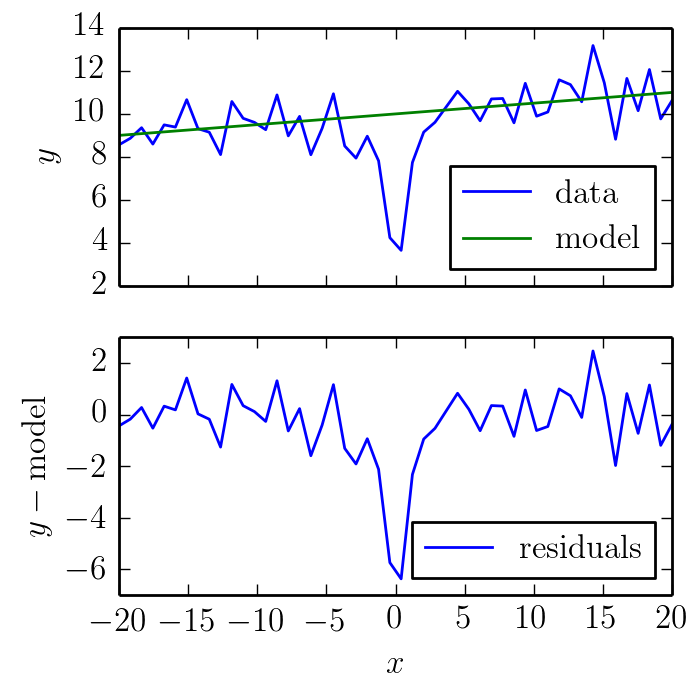
\includegraphics[width=0.5\textwidth]{fake_line}
\caption{A fake Gaussian residual resulting from an imperfect model.}
\label{fig:fake_line}
\end{center}
\end{figure}

\begin{figure}[!htb]
\begin{center}
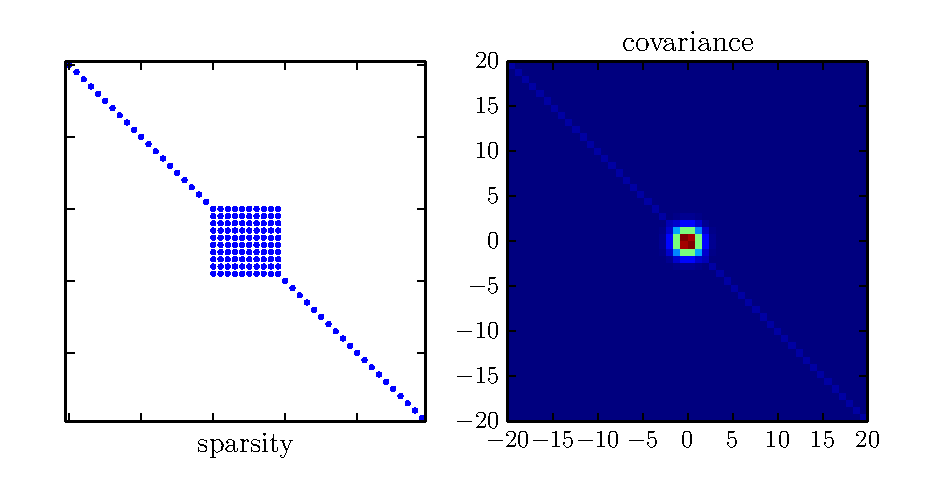
\includegraphics{matrix_region}
\caption{Covariance matrix of a single patch of Gaussian noise. Left: sparsity diagram. Right: covariance matrix.}
\label{fig:matrix_region}
\end{center}
\end{figure}

\begin{figure}[!htb]
\begin{center}
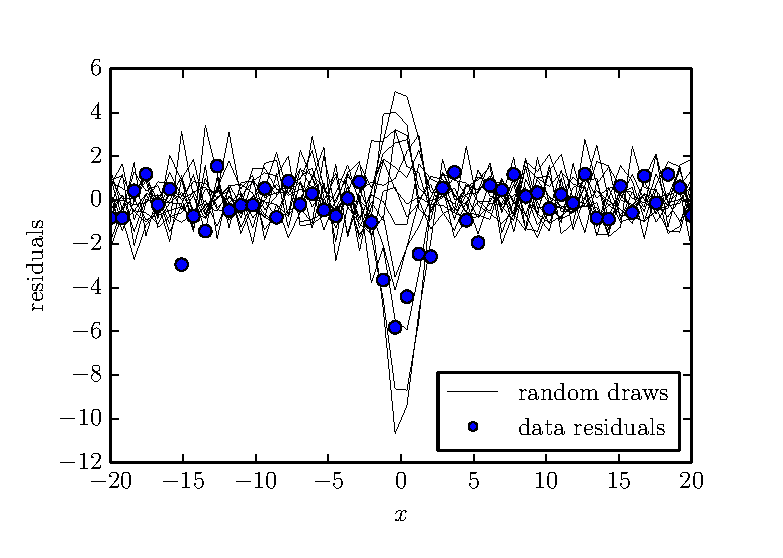
\includegraphics{random_draw}
\caption{15 random draws from the covariance matrix, overplotted with the residuals from Figure~\ref{fig:fake_line}.}
\label{fig:random_draw}
\end{center}
\end{figure}

\subsection{Global covariance}
DFM recommended that we also implement a stationary covariance kernel to account for the general covariance structure of the data. For this, we use a Matern kernel 
\begin{equation}
  k_{\nu = 3/2}(r, a, l) = a \left(1 + \frac{\sqrt{3} r}{l} \right ) \exp \left (- \frac{\sqrt{3} r}{l} \right ) 
\end{equation}
and add compact support by tapering with a Haan window
\begin{equation}
  w(r) = 0.5 + 0.5 \cos \left( \frac{\pi r}{r_0} \right)
\end{equation}
This kernel does a decent job of matching the covariance structure that still remains in a region of stellar continuum. We sample the parameters describing these kernels in our MCMC code. We also have a bit of logic that adds the patches of correlated noise until we have addressed all of the egregious residuals.

\hcom{good on the stuff about there being important information where the models and data disagree.}

I am fairly new to the Gaussian processes kernel game, but I would imagine that different covariance functions could be useful for different spectral problems, such as M dwarf continuua (Figure~\ref{fig:mann}). My first attempt is to create a new kernel with a finite bandwith taper to replace the original Gaussian kernel for a bad spectral line. This covariance function is a squared exponential with a Gaussian taper
\begin{equation}
k(x, x^\prime | h, a, \mu, \sigma) = \exp \left ( \frac{-( x - x^\prime)^2 }{2 h^2} \right ) \frac{a^2}{2 \pi \sigma} \exp \left ( - \frac{[(x - \mu)^2 + (x^\prime - \mu)^2]}{2 \sigma^2}\right )
\end{equation}
here $h$ is a "bandwidth" that controls the power of the oscillations. If $h$ is small, then there will be high-frequency structure (such as in an M dwarf residual). If $h$ is large, then only low-frequency structure will remain (such as in an FGK residual).

\begin{figure}[!htb]
\begin{center}
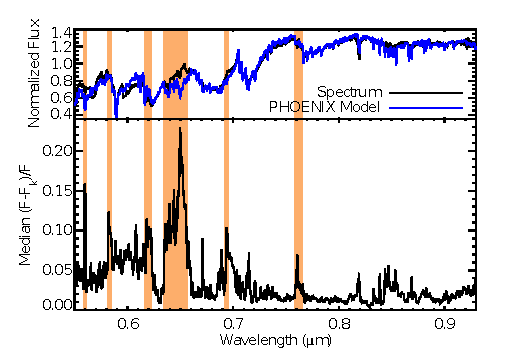
\includegraphics{mann}
\caption{Figure from \citet{mga13} showing the residuals (bottom panel) commonly encountered when fitting M dwarf spectra.}
\label{fig:mann}
\end{center}
\end{figure}


\hcom{in your four classes of line behavior, there is none which is dominated by continuum issues? Or is there? That is, continuum fitting can cause problems, no?}
In principle, there should be areas where continuum fitting can be a problem. However, in the stars I'm looking at (over a narrow echelle range), the Chebyshev formalism essentially assumes that any continuum mis-match is actually a flux-calibration (instrumental) issue, and accounts for it. This means that if we were fitting hotter stars with few lines, any information contained in the continuum shape would be lost. 

\hcom{Section 5: You might even be able to learn changes to the models. This is the holy grail.}

If we were to run against a large spectroscopic library of many stars (say, the \emph{Kepler} follow-up sample, or some SLOAN sample), we could use the learnt covariance of the spectrum to identify the bad regions and then determine how the models would need to be changed in order to fit all of the observed stars the best, similar to using Gaussian processes to predict the value of a function where data is missing. 

\section{Chebyshev}
\hcom{Can you really marginalize analytically over the Chebyshev polynomials? And doesn't that make a huge, correlated uncertainty tensor? And what priors do you use?}
\hcom{In re +/- 0.01 dex: You have tons of pixels so of course you get amazing constraints! It would be surprising if you didn't. But do you get such amazing constraints if you marginalize analytically over thousands of Chebyshevs?}
Because the residual echelle blaze is smooth and small ($\le 5\%$ error) we use only a fourth-order Chebyshevs to fit each order of the spectrum. For a visual description of what this looks like in practice, please see \url{http://iancze.github.io/image.html}.


\bibliography{disks,bayesian,master}
\bibliographystyle{hapj}
\end{document}
